
\renewcommand{\thechapter}{3}
\chapter{The Lightmap}

The EXO detector was designed with roughly 450 APDs ganged into 74 channels of six to seven APDs each.  These APDs were set into the two endcaps of the cylindrical EXO detector.  Three of the APD ganged channels were disabled due to noisy components before physics data collection began; a fourth channel was disabled in February 2012 due to increasing noise in its components.  Additional stepwise changes in APD behavior come from changes to the electronics which have been implemented multiple times during the course of the experiment.

The different positions of the APDs means that given the same amount of energy deposited into the detector, a channel may show a larger or smaller signal depending on the location of the energy deposit.  Additionally, there will be time-dependent changes: gain will drift in each APD at independent rates, and stepwise changes to the APD signals comes from changes to electronics and disabling of channels.

As a result, when we attempt to characterize the APD response of our detector, it is critical to map out the time and space dependence of that response.  Early attempts to do this focused on periodic campaigns to collect large amounts of known-energy data and characterize the APD response at a moment in time.  These campaigns would generally consist of days of source data.  The strong Thorium source would be used, and an expert would be on-site to position the source in a wide range of locations, to ensure that a single campaign was independently sufficient to characterize the APD response.  The 2615-keV single-site gamma line of the Thallium 208 daughter product of Thorium 228 was isolated in offline analysis, and signals from these events were used to measure the signal magnitude from a known-energy single-position deposit in the detector.

Even with such a significant quantity of source data, statistics were found to be insufficient.  Some regions of the detector were difficult to illuminate, and signals on individual channels were small.  To simplify the problem, signals on each endcap were summed together (without gain corrections) so that the 70 or 71 active APD channels could be treated as two large-magnitude APD channels instead.  This increased the size of the signals; it also made the spatial dependence of the response smoother, so that a sparser distribution of data can still be sufficient to characterize the response.  This permitted the creation of an APD-plane lightmap which allowed EXO to produce its first position-dependent corrections to scintillation energy.

Although the APD-plane lightmap produced significant improvements in the energy resolution achieved by the EXO detector, inevitably it was only an incomplete characterization of the APD response.  Indeed, because for $\beta\beta0\nu$ studies we place our fiducial cut as close to the edges of the detector as possible, in certain regions of the detector our scintillation signal might be highly concentrated on one or a small number of channels.  Summing together multiple channels is, in this sense, a lossy form of compression of the data, and it is tempting to see whether we can extract better physics if it is avoided.  Thus, characterizing the APD yield on individual APD-gang channels is not in itself an important component of our analysis, but may be expected to provide a critical tool for more advanced scintillation analysis.

\section{Four-Dimensional Lightmap}

\begin{figure}
\begin{center}
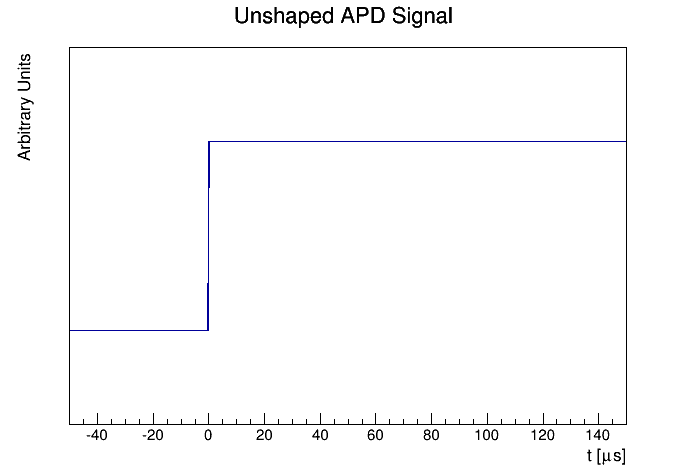
\includegraphics[keepaspectratio=true,width=\textwidth]{scripts/UnshapedAPDWaveform.png}
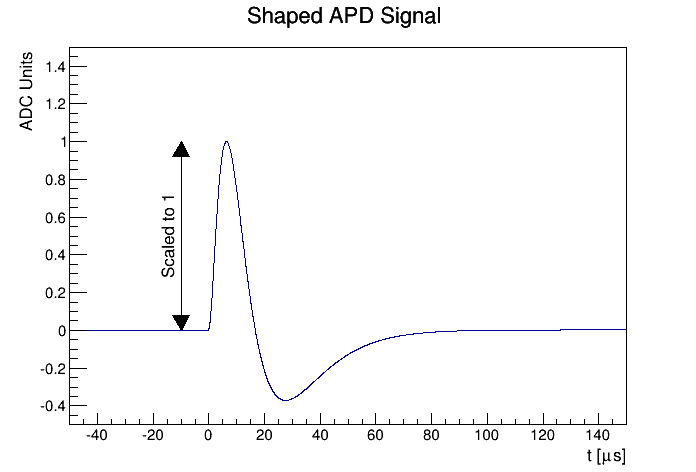
\includegraphics[keepaspectratio=true,width=\textwidth]{scripts/ShapedAPDWaveform.png}
\end{center}
\renewcommand{\baselinestretch}{1}
\small\normalsize
\begin{quote}
\caption{Shaped and unshaped APD waveforms.  The normalization is shown to make the peak of the shaped waveform have a magnitude of one, and the time axis is shifted so that the unshaped waveform is a step function centered at $t=0$.}
\label{fig:SampleAPDTemplates}
\end{quote}
\end{figure}
\renewcommand{\baselinestretch}{2}
\small\normalsize

As described above, in constructing an individual-APD lightmap we face two conflicting needs: we must use as much data as possible to handle the faster spatial dependence and smaller signals expected, but if too much data is included then we run the risk of combining data taken when an APD had a different gain.  If we truly wish to use all available data, then we will need to simultaneously understand the full time-dependence of the gain.  In other words, rather than forming a small number of independently-measured three-dimensional lightmaps, we will need to measure a four-dimensional lightmap $L(x,y,z,t)$.  Since we will use Thorium-226 source data to generate the lightmap, we require that our lightmap should predict the magnitude of the signals on each APD gang induced by a single-site deposit of energy $2615$ keV; figure~\ref{fig:SampleAPDTemplates} shows our definition of a unit-magnitude signal.

This may at first seem infeasible.  After all, by adding an independent time argument it appears that rather than measuring a lightmap independently from each calibration campaign, we must measure one independently for each time bin.  But we can make a key simplifying assumption that the lightmap is separable.  In a physical sense, we can assume that:
\begin{enumerate}
\item From a given position $(x,y,z)$ photons deposit on each APD channel at a constant rate.
\item Each APD channel in turn magnifies and shapes its signal with a gain which may vary in time, but does not depend on the point of origin of the photons.
\end{enumerate}
So, we demand that the lightmap have the much simpler form
\begin{equation} \label{eq:SeparableLightmap}
L(x,y,z,t) = R(x,y,z)S(t)
\end{equation}

Is this simplification fully motivated by the detector?  It must be admitted that it is not.  The first point is fairly accurate:  we must trust that the electric field and the reflectivity of detector surfaces are constant in time, but basically these conditions are assumed to hold within EXO-200.

However, each channel can draw its signal from multiple APDs, each of which has an independent time-varying gain.  Photons from a deposit may preferentially sample the gain from the closest APD within a channel, so deposits in different locations may track more closely the gain of the closest APD within a channel, and the second point may not be accurate.  Studying the impact of this effect should be a topic for future study, particularly to understand to what degree it limits the effectiveness of a lightmap; it may be relevant to nEXO planning to understand how ganging together APDs limits scintillation resolution.  Currently it is assumed to be a small effect and ignored.

So, treating equation ~\ref{eq:SeparableLightmap} as valid, one simple general scheme to find $R$ and $S$ iteratively is:
\begin{enumerate}
\item \label{item:FormingListOfHits} Compile, as well as possible, a list of single-site 2615-keV events from Thorium-228 source data.  Some Compton-scattered events will inevitably leak into this dataset, but the selection criteria should be designed to minimize this leakage while maximizing the fraction of true 2615-keV events accepted.
\item Initially, assume a constant function $S(t) = 1$ for all APD channels.
\item \label{item:ReentryForLightmapAlg} For each APD channel, estimate $R(x,y,z) = L(x,y,z,t)/S(t)$ from the set of events tabulated in step ~\ref{item:FormingListOfHits}.
\item For each APD channel, estimate $S(t) = L(x,y,z,t)/R(x,y,z)$ from the set of events tabulated in step ~\ref{item:FormingListOfHits}.
\item If convergence has not yet been reached, return to step ~\ref{item:ReentryForLightmapAlg}.
\end{enumerate}
Although this algorithm is not necessarily guaranteed to achieve convergence at all, in practice $S(t)$ is close to constant, resulting in fairly rapid convergence.

\section{Algorithm Details}

The previous section outlines a general algorithm for computing a four-dimensional lightmap from source data.  In this section I will specify the implementation choices which are made in the code currently being used.  In attempt to encourage future experimentation, alternative options will also be listed in some detail, along with some motivations for these alternatives.  Time has not permitted testing of all of these options, but it is hoped that they will be explored in the future.

\subsection{Event Selection}

The single-site Thorium-228 spectrum is well-peaked at 2615 keV, making it an excellent monoenergetic calibration line.  Our challenge is to select truly 2615-keV events as efficiently as possible, while simultaneously avoiding near-2615-keV events which may leak into the dataset.

This is an inherently iterative process.  The first lightmap had to be constructed from an ionization-only spectrum because no useful position-corrected scintillation measurement existed; the resolution of the ionization-only spectrum was quite poor, roughly $3.5\%$ (sigma) of the energy, as described in Steve Herrin's thesis, and severe compromises had to be made to keep the Compton-shoulder leakage down to acceptable levels.  That work required events to have ionization between $0.33\sigma$ and $3\sigma$ to the right of the ionization peak.~\cite{ThesisSteve}

Such a strongly asymmetric cut was chosen to avoid leakage from compton shoulder events, which it did successfully.  However, because of anticorrelation between scintillation and ionization, choosing events whose ionization had oscillated high means this cut was also preferring events whose scintillation had oscillated low, introducing a bias in the lightmap magnitude.  Additionally, the cut permits less than $37\%$ of desired events to be accepted, which is a substantial loss of efficiency that has a significant impact in certain low-statistics regions of the detector.

The current work has had the benefit of an existing position-corrected scintillation measurement, leading to a rotated energy spectrum with resolution of roughly $1.8\%$.  As a result, it is possible to accept a wider cut (in sigmas) while still keeping Compton shoulder leakage small.  We currently accept all events within $2\sigma$ of the peak, with better than $95\%$ acceptance and only small leakage.  An additional benefit is that this improved resolution allows us to use a symmetric acceptance region, avoiding the implicit bias introduced from the earlier asymmetric cut window.

Preliminary investigations have been conducted to see what impact is observed from using the denoised scintillation measurements which are the subject of this work.  Presently the improvement in resolution (to roughly $1.4\%$) has not demonstrated any significant improvement in the quality of the lightmap; however, this is a topic of continuing study which will certainly be revisited.

Beyond the cuts described above (single-site within an appropriate energy window), other basic cuts are applied to ensure only well-behaved scintillation signals are selected:
\begin{itemize}
\item Charge and light must individually lie within a reasonable range.
\item The charge-to-light ratio must not identify an event as an alpha decay.
\item The scintillation time must be well-separated from any other scintillation signals in same event frame.
\item All charge signals which are assigned to this scintillation signal must be assigned unambiguously.
\item All three position coordinates must be known.  (No fiducial cut is placed, since that would restrict the volume where the lightmap is specified.)
\end{itemize}
Many of these cuts are probably no longer necessary -- as the resolution has improved, the chances of contamination have decreased and we can be a bit less cautious about accepting events.  It is worth remembering, though, that our main analysis only accepts events with a single scintillation signal, something which we cannot afford to do.  (The statistics from strong Thorium source runs are too valuable, particularly because they are the primary source of statistics in some regions of the detector.)  As a result, it is important to maintain some caution with cuts designed to handle those events more robustly.

\subsection{Function Parametrization}

Because we are attempting to empirically measure the functions $R(x,y,z)$ and $S(t)$ from a finite dataset, we need to specify some more limited form for them to take.  All current approaches to describing $R(x,y,z)$ first bin the detector volume into three-dimensional voxels, and then define $R(x,y,z)$ to interpolate linearly between known values at the center of the voxels.  The size of these voxels must be chosen with some care; if they are too small, then low per-voxel statistics will cause the statistical errors on the signal magnitude to dominate, whereas if the voxels are too large then the spatial variation of the lightmap will not be fully captured.

In the current lightmap, the detector is binned into $1 cm^3$ voxels; the detector is easily contained within a box with sides $40 cm$ long, leading to $64,000$ voxels (many of which lie outside the detector and will be empty).  The choice of voxel size was made based on the size of an individual APD.  The APDs are roughly $2.5 cm$ in diameter, so very near the anode we would like for the size of a voxel to be much smaller than $2.5 cm$.  When this is done, much of the detector has entirely sufficient statistics per voxel; however, there are some regions of the detector with fewer than ten hits per voxel, indicating that these regions may have quite significant statistical error.

It is possible to justify a choice of larger voxels.  The APDs lie at $\pm 204 mm$ from the cathode, which means that there is more than $1 cm$ (WHAT IS IT?) between our fiducial volume and the APDs.  At this distance, the dependence of the lightmap on $x$ and $y$ is expected to be much slower than at the APD plane, indicating that perhaps $2 cm$ binning in $x$ and $y$ may be sufficient.  Additionally, $z$-dependence of the lightmap is expected to be fairly smooth throughout the detector; since we interpolate linearly between voxels, it may be possible to use a $z$-binning much coarser than $1 cm$.  This may be a topic for future investigation.

It is also worth mentioning that less intuitive voxel geometries have been tried in the past.  The older APD-plane lightmap~\cite{ThesisSteve} used a cylindrical-coordinate binning; binning in $r$ was selected to make the bin volumes roughly constant along the $r$ axis, binning in the angular coordinate was uniform, and binning in $z$ was chosen to be coarser near the anodes and finer near the cathode to reflect faster variation there.  In all cases the binning is coarser than with the current cubic voxels being used; this is made possible by the larger quantity of available statistics from running much longer, and is justified by the potential for the yield on a single APD gang to vary more rapidly than the yield averaged across an entire APD plane.

It is well-known~\cite{MultivariateDensityScott} that when it is necessary to estimate a multivariate function from limited statistics, a choice of binning can have a significant impact on the result.  It is preferable to use an unbinned technique such as kernel regression.  In particular, our data density is highly non-uniform, and it should be possible to measure the lightmap which high fidelity in regions of high statistics, while smoothly transitioning to a coarser interpolation in regions of low statistics to minimize the impact of uncertainty from individual hits.  State-of-the-art solutions to this problem would rely on locally adaptive kernel regression; see ~\cite{MultivariateDensityScott} for a detailed explanation of the related issues in kernel estimation.  (SHOULD HAVE A CHAPTER ON REGRESSION AS WELL -- BUT UNFORTUNATELY LEFT IT IN THE OFFICE, AND CAN'T ACCESS ONLINE.  RETURN TO THIS.)  Attempting to use a locally adaptive kernel regression for $R(x,y,z)$ should be considered a highly appealing extension to the algorithm for generating a lightmap.

The parametrization of $S(t)$ presents a very different set of choices.  Thorium data is taken in bursts, with the time between mostly filled by low-background runtime.  When we choose to treat $S(t)$ as a smoothly varying function, it becomes critical to interpolate properly -- after all, the low-background runtime is the critical part of the experiment.  (If we only produce a lightmap accurate during source runtime, we will measure an energy resolution from source data which is not borne out in the low-background data, so we should in fact be able to give some guarantee that $S(t)$ is almost as accurate during the low-background runtime as during the source runtime.)  Fortunately, it is generally true that the time variation of the APD response is quite slow; exceptions are generally due to changes in the electronics which should occur at well-specified times.

Currently each source run is treated as a burst of data taken at the midpoint of the run, and $S(t)$ is measured at that point only from the data of that run; then $S(t)$ is linearly interpolated between those points.  In principle it is possible that between two source runs an electronics change may have been performed, which would mean that a better interpolation would be to assume $S(t)$ is flat except for a step at the time of the electronics change; in practice, though, it has generally been the practice of the collaboration to take a source run immediately before and after an electronics change, so no high-value data is taken during that interval and this detail can be ignored.

Another concern with this method is what should be done with short source runs.  If a run is too short, then the measurement of $S(t)$ coming from that run may have significant errors.  We currently mitigate this issue by entirely throwing out all data from runs with fewer than $100$ usable events.  We justify this approach by claiming that even though those events might in principle have contributed some useful information on $R(x,y,z)$, without a good measurement of the relevant $S(t)$ it is impossible to use that data.

It would be better if we made use of our knowledge that $S(t)$ changes slowly or at well-defined moments.  In the future, it would be useful if instead we performed smoothed interpolations between electronics changes.  This could be done in the same style as EXO's lifetime corrections, using polynomial fits, where the degree of the polynomial could be determined by eye.

Alternatively, often there will be a long string of consecutive source runs which should be combined into one higher-statistics dataset.  This process would need to be done essentially by hand, and has not been performed for the current analysis, but it could benefit the accuracy of the $S(t)$ function and also recover some statistics in cases where the individual runs might be too short for inclusion in the lightmap dataset.

The choice of binning or parametrization for $R(x,y,z)$ and $S(t)$ can have a profound impact on the accuracy of the lightmap, and the current analysis has only skimmed the surface in trying options.  It is hoped that further work on the lightmap will include significant investigation in these topics.

\subsection{Convergence and Error Estimation}

The topics of convergence and error estimation for the lightmap are perhaps the most rudimentary; a full analysis of the lightmap cannot be complete without them.  However, for the current analysis they are approached essentially by a series of guesses; the lightmap is then used in further analysis, and the validity of the lightmap is established by its successful use in that downstream work.

Error estimation is not attempted on the current lightmap.  We do study the number of hits observed in each position voxel of the detector (see section ~\ref{sec:LightmapVisualization}), and presume that the most significant source of error comes from low-statistics regions of the detector.  However, no explicit estimation of the lightmap uncertainty has been attempted.

One difficulty with estimating the errors in the lightmap function $L(x,y,z,t)$ comes from the correlation between errors in $R(x,y,z)$ and $S(t)$.  If one of those two components were known perfectly, then we could treat the fit uncertainties of each hit as independent errors, and propagate those errors into an uncertainty for each voxel of $R(x,y,z)$ (if $S(t)$ is assumed to be perfectly known) or $S(t)$ (if $R(x,y,z)$ is assumed to be perfectly known).  But in reality, all of the measurements of $R(x,y,z)$ are correlated with all of the measurements of $S(t)$, meaning that even the errors of different voxels of $R(x,y,z)$ or different times in $S(t)$ are correlated with each other.  Fully characterizing these errors could evolve into a significant project in itself, and it is not clear that the payoff could justify such an investment of effort or computation.

Although a full estimate of lightmap errors with correlations would probably be computationally quite intensive to produce, it might be possible to estimate the independent errors of each voxel of the position lightmap $R(x,y,z)$ or each independent run making up $S(t)$ by treating the other function as perfectly known, as described above.  This would generally produce an underestimate of the uncertainty in each, but the estimate might still give some benefit.

To produce a more accurate estimate of errors, it would probably be necessary to do a simultaneous fit by varying both $R(x,y,z)$ and $S(t)$ together.  In the current scheme, $R(x,y,z)$ contains far more complexity than $S(t)$ with roughly $50,000$ non-empty voxels, so for each APD gang we would need to simultaneously vary roughly $50,000$ parameters to obtain the optimal lightmap.  It is exactly this time-intensive process which was avoided by choosing the iterative approach for measuring the lightmap; however, this is still the sort of problem which is routinely managed in large-scale applications, and it would only need to be solved occasionally when it is necessary to derive a new lightmap, so it is not infeasible to imagine attempting it.  The prospect of feeding in a high-quality guess obtained from the iterative method presents an additional significant time-saver.  This method would not fully account for the correlations between errors of the different voxels of $R(x,y,z)$ or runs in $S(t)$, but it would come closer than the previous naive method.

However, it is also possible that identifying the error of each voxel or run is heading down the wrong path.  As described earlier, it is likely that the optimal (lowest-error) method for estimating the lightmap will be an unbinned method such as a locally-adaptive kernel regression method.  Error estimation in kernel regression presents significant additional challenges compared to errors from binned parametrizations.  At present, I am not aware of any simple scheme to manage this difficulty, meaning that there may be the paradoxical tradeoff that the best method for minimizing lightmap errors simultaneously makes those errors infeasible to estimate.

Note that under the iterative method, the most naive method for estimating errors is not valid.  It might appear that when $S(t)$ is initialized to a constant value of $1$, we could also assign to it some constant error.  Then when we compute $R(x,y,z)$, we could propagate independent errors from the fit uncertainties of signals and from $S(t)$; and when we compute $S(t)$ we could propagate independent errors from the fit uncertainties and from $R(x,y,z)$; and so forth.  However, such a scheme provides no compensating feedback mechanism to force the iterated errors to a reasonable or accurate value, so there is no reason to believe the errors from such a system (if, that is, they converge at all).  This difficulty may underscore the fundamental challenge associated with measuring the lightmap errors within our scheme -- iterative methods are well-suited to solving a system, but when correlated errors are mistreated as uncorrelated an iterative method can easily magnify the impact of that mistreatment.

On the topic of convergence, it has been mentioned already that by starting with a generally accurate initial guess for $S(t)$ as constant, the iterative solution method tends to converge rapidly.  As a result, and because iterations take only a few hours to perform, we currently perform three to four iterations and claim that convergence is generally roughly reached.  Ideally, we would require that none of the position voxels or runs change value within an iteration by more than some fraction of their estimated errors; but in the absence of estimated errors, this is of course impossible.

It would be possible, in a conservative approach, to require each value to converge to some small fraction of an ADC unit, ensuring that the convergence is better than our ability to measure signals.  Such a requirement might force us to compute more iterations than are truly warranted by our lightmap errors, but given the reasonable speed of each iteration, such a method still might not be unreasonable.  


\section{Visualization} \label{sec:LightmapVisualization}

\begin{figure}
\begin{center}
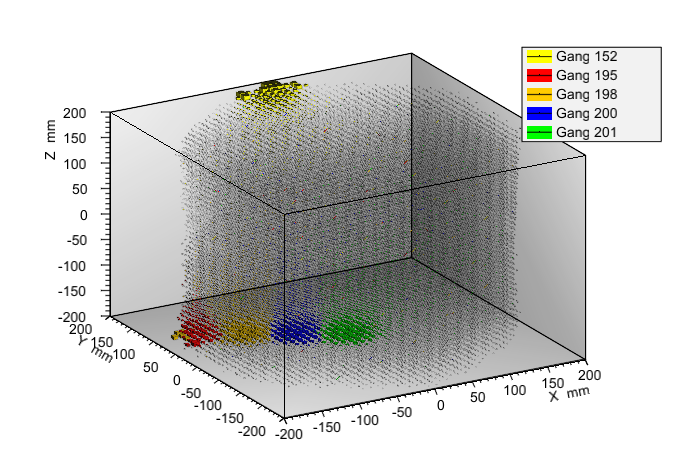
\includegraphics[keepaspectratio=true,width=\textwidth]{Lightmap_viz.png}
\end{center}
\renewcommand{\baselinestretch}{1}
\small\normalsize
\begin{quote}
\caption{Lightmap position-dependence $R(x,y,z)$ for selected APD gangs.}
\label{fig:Lightmap3DPlot_unzoomed}
\end{quote}
\end{figure}
\renewcommand{\baselinestretch}{2}
\small\normalsize

\begin{figure}
\begin{center}
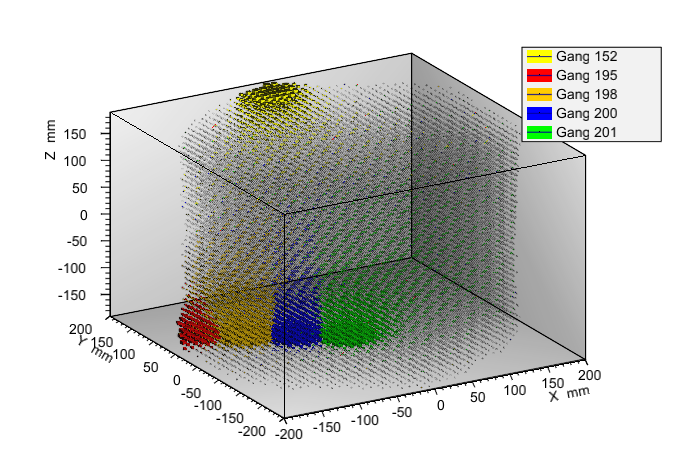
\includegraphics[keepaspectratio=true,width=\textwidth]{Lightmap_viz_zoom.png}
\end{center}
\renewcommand{\baselinestretch}{1}
\small\normalsize
\begin{quote}
\caption{Lightmap position-dependence $R(x,y,z)$ for selected APD gangs.  Here extreme anode positions are omitted to permit better contrast for the lightmap in the fiducial volume.}
\label{fig:Lightmap3DPlot_zoomed}
\end{quote}
\end{figure}
\renewcommand{\baselinestretch}{2}
\small\normalsize

\begin{figure}
\begin{center}
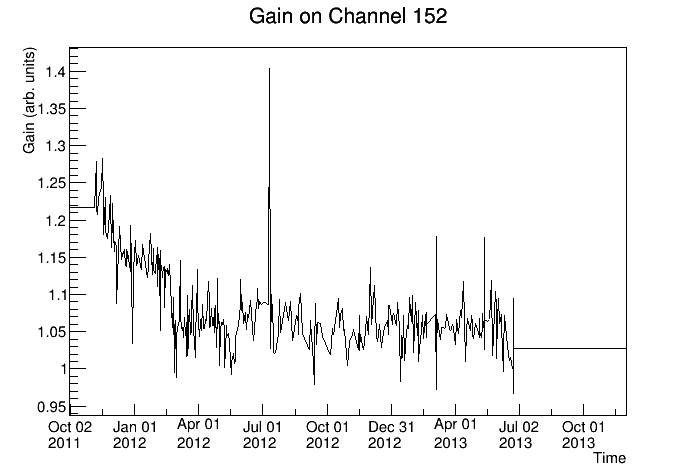
\includegraphics[keepaspectratio=true,width=\textwidth]{gainfunc_152.png}
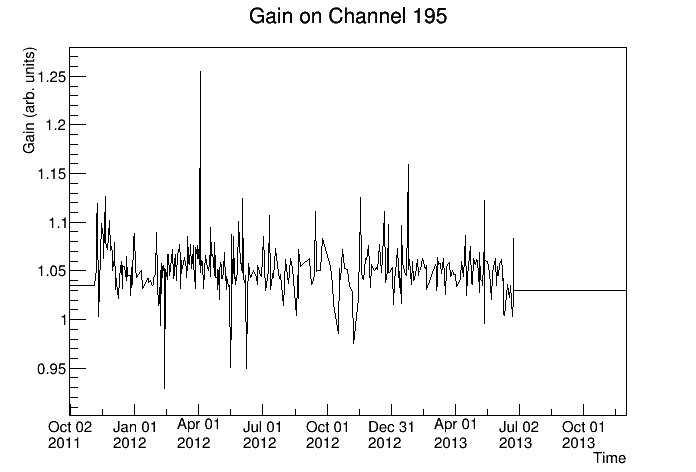
\includegraphics[keepaspectratio=true,width=\textwidth]{gainfunc_195.png}
\end{center}
\renewcommand{\baselinestretch}{1}
\small\normalsize
\begin{quote}
\caption{Functions $S(t)$ for selected channels.}
\label{fig:LightmapGainFunc1}
\end{quote}
\end{figure}
\renewcommand{\baselinestretch}{2}
\small\normalsize

\begin{figure}
\begin{center}
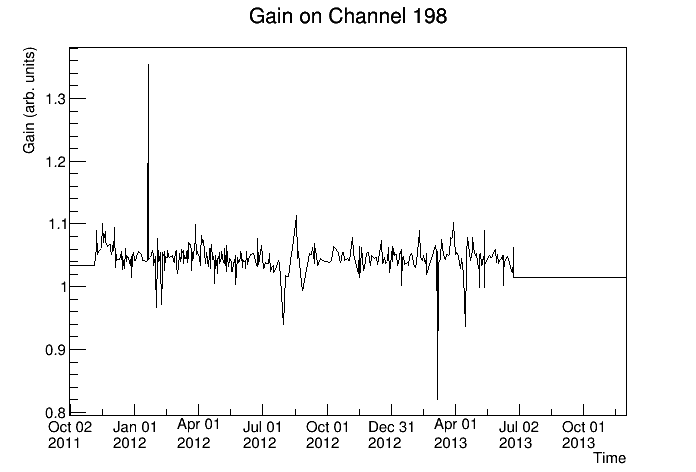
\includegraphics[keepaspectratio=true,width=\textwidth]{gainfunc_198.png}
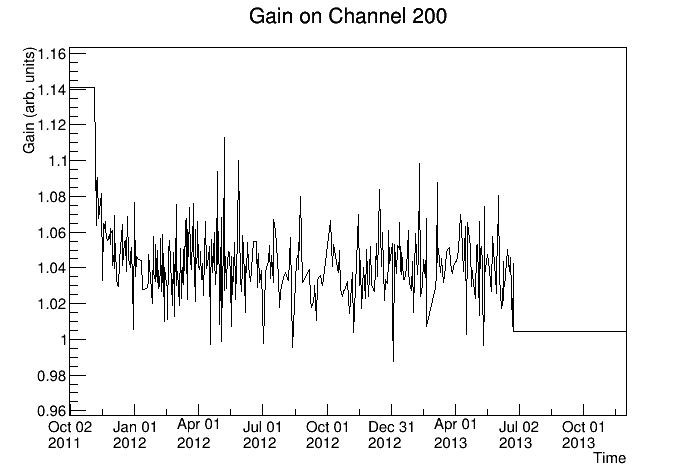
\includegraphics[keepaspectratio=true,width=\textwidth]{gainfunc_200.png}
\end{center}
\renewcommand{\baselinestretch}{1}
\small\normalsize
\begin{quote}
\caption{Functions $S(t)$ for selected channels.}
\label{fig:LightmapGainFunc2}
\end{quote}
\end{figure}
\renewcommand{\baselinestretch}{2}
\small\normalsize

\begin{figure}
\begin{center}
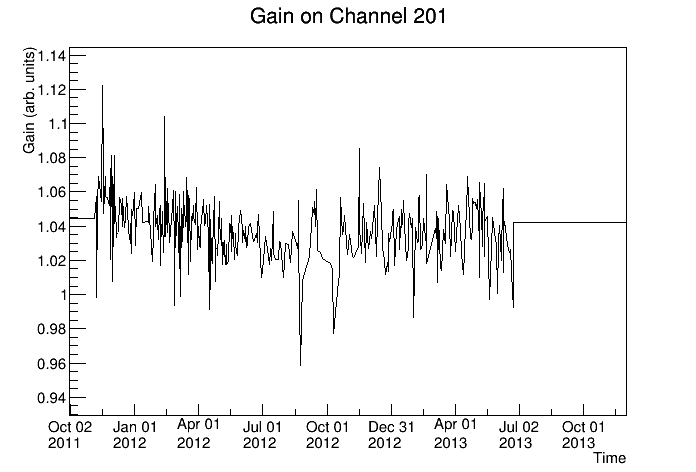
\includegraphics[keepaspectratio=true,width=\textwidth]{gainfunc_201.png}
\end{center}
\renewcommand{\baselinestretch}{1}
\small\normalsize
\begin{quote}
\caption{Functions $S(t)$ for selected channels.}
\label{fig:LightmapGainFunc3}
\end{quote}
\end{figure}
\renewcommand{\baselinestretch}{2}
\small\normalsize

Although it is not strictly necessary to be able to visually inspect the lightmap for it to be useful, nevertheless it is reassuring to see that the lightmap is qualitatively similar to intuitive expectations of how light should propagate through the detector.  We have chosen to store the position-dependent $R(x,y,z)$ for each APD gang as a set of ROOT TH3D objects, and fortunately ROOT provides a number of excellent plotting features suitable for a three-dimensional dataset.  In figure~\ref{fig:Lightmap3DPlot_unzoomed}, it is possible to view the values of $R(x,y,z)$ for a sample of gangs on top of each other.  Larger boxes and denser color indicates a higher yield on the APD gang in question, and it is immediately apparent that events near the anodes produce light which is highly concentrated on a single APD gang.

Figure~\ref{fig:Lightmap3DPlot_unzoomed} shows the highest yield on the very boundary of the detector, well outside of our fiducial volume; to permit us to more easily view contrast inside of the detector, figure~\ref{fig:Lightmap3DPlot_zoomed} shows the same map while omitting the most extreme bin near either anode.  Viewing this map, we can see more interesting characteristics of the lightmap:
\begin{itemize}
\item Events near the anodes show a high signal concentration on the one gang nearest to their position; however, even deep into the detector near the cathode it is still possible to see the higher concentration of signal on the gang directly aligned with the event.
\item We can also see, from gang 201 (green), that events can produce significant signal on APD gangs which which they are not directly aligned (in the Z direction); yield on gang 201 can be seen to decrease smoothly in all directions.
\item APD gangs in the corners of the detector, such as gang 195 (red), are not effective at measuring light from events which are far away; even directly above gang 195, it is clear that gang 198 is more effective at collecting light farther away than about five to ten centimeters.
\end{itemize}

ALSO TALK ABOUT GAIN VS. TIME, HITS PER VOXEL, OTHERS?


\section{Implications for Signal Reconstruction}

Prior to this work, it was standard to sum all of the scintillation waveforms from gangs on a single anode plane.  The lightmap we have produced provides a trove of information about how light propagates through the detector, and as such it can be used to identify qualitatively how scintillation signal reconstruction might be improved.

Most significantly, figure~\ref{fig:Lightmap3DPlot_zoomed} demonstrates that 









